\newpage
\section{PROCEDIMIENTO}
\begin{enumerate} [label={\alph*.}]
    \item Armar el circuito oscilador diseñado, comprobar su frecuencia y amplitud de salida.
    \begin{figure}[H]
        \centering
        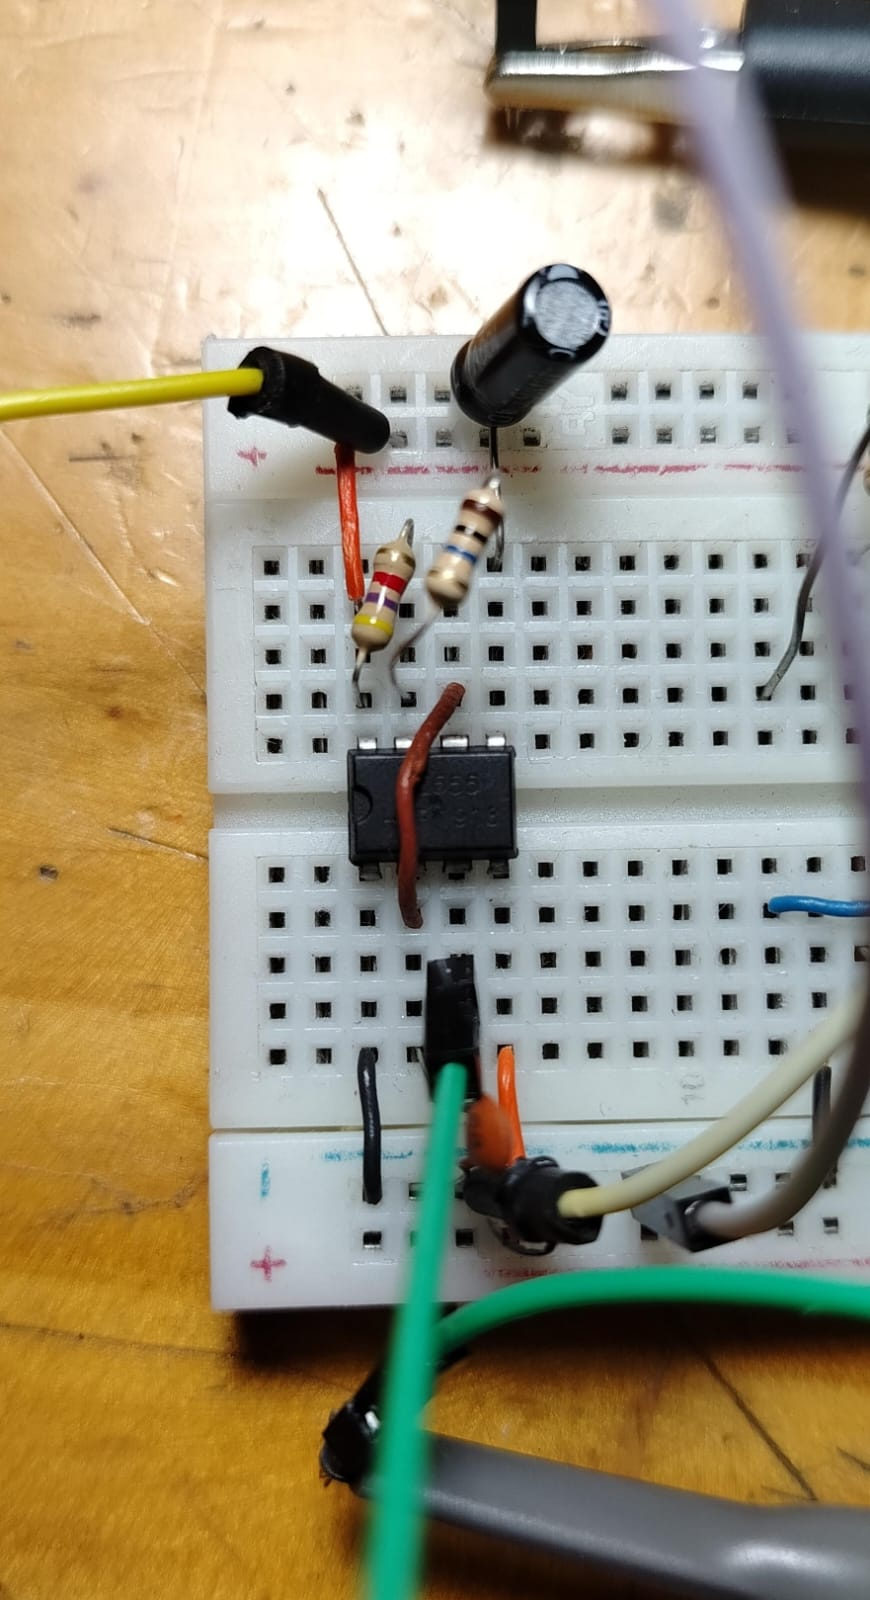
\includegraphics[width=.35\textwidth]{imgs/5.1. Circuito.jpg}
        \caption{Oscilador con NE555}
    \end{figure}
    \begin{figure}[H]
        \centering
        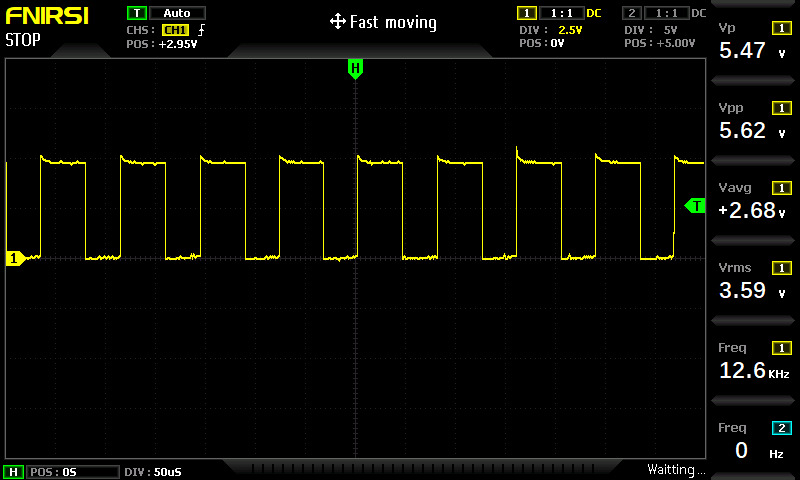
\includegraphics[width=.9\textwidth]{imgs/5.1. Osciloscopio del circuito.jpg}
        \caption{salida del oscilador}
    \end{figure}
    \item Armar el circuito de la Fig. 2, aplicar la señal de salida del oscilador, alimentar el circuito y observar la señal de salida en el osciloscopio.
    \begin{figure}[H]
        \centering
        \includegraphics[width=.9\textwidth]{imgs/5.2. CIrucito.jpg}
        \caption{Sintetizador con un PLL y un 7493}
    \end{figure}
    \begin{figure}[H]
        \centering
        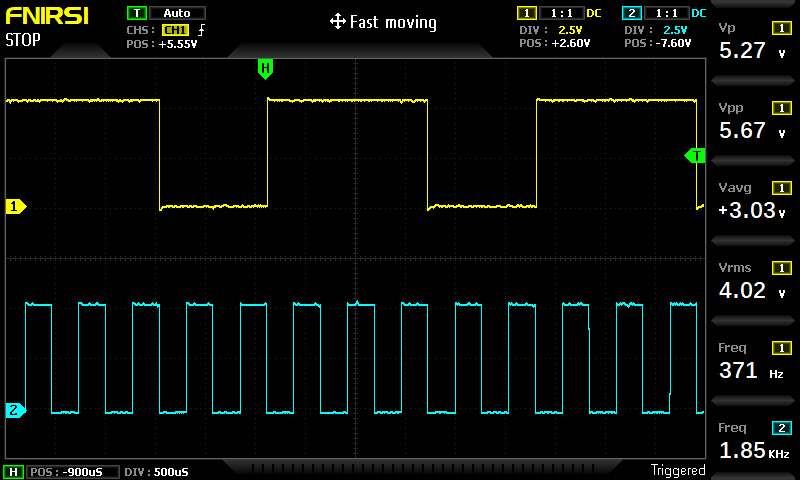
\includegraphics[width=.9\textwidth]{imgs/5.2. Salida del circuito.jpg}
        \caption{Comparación entre la entada del demodulador de fase y el VCO (división x4)}
    \end{figure}
    \newpage
    \begin{figure}[H]
        \centering
        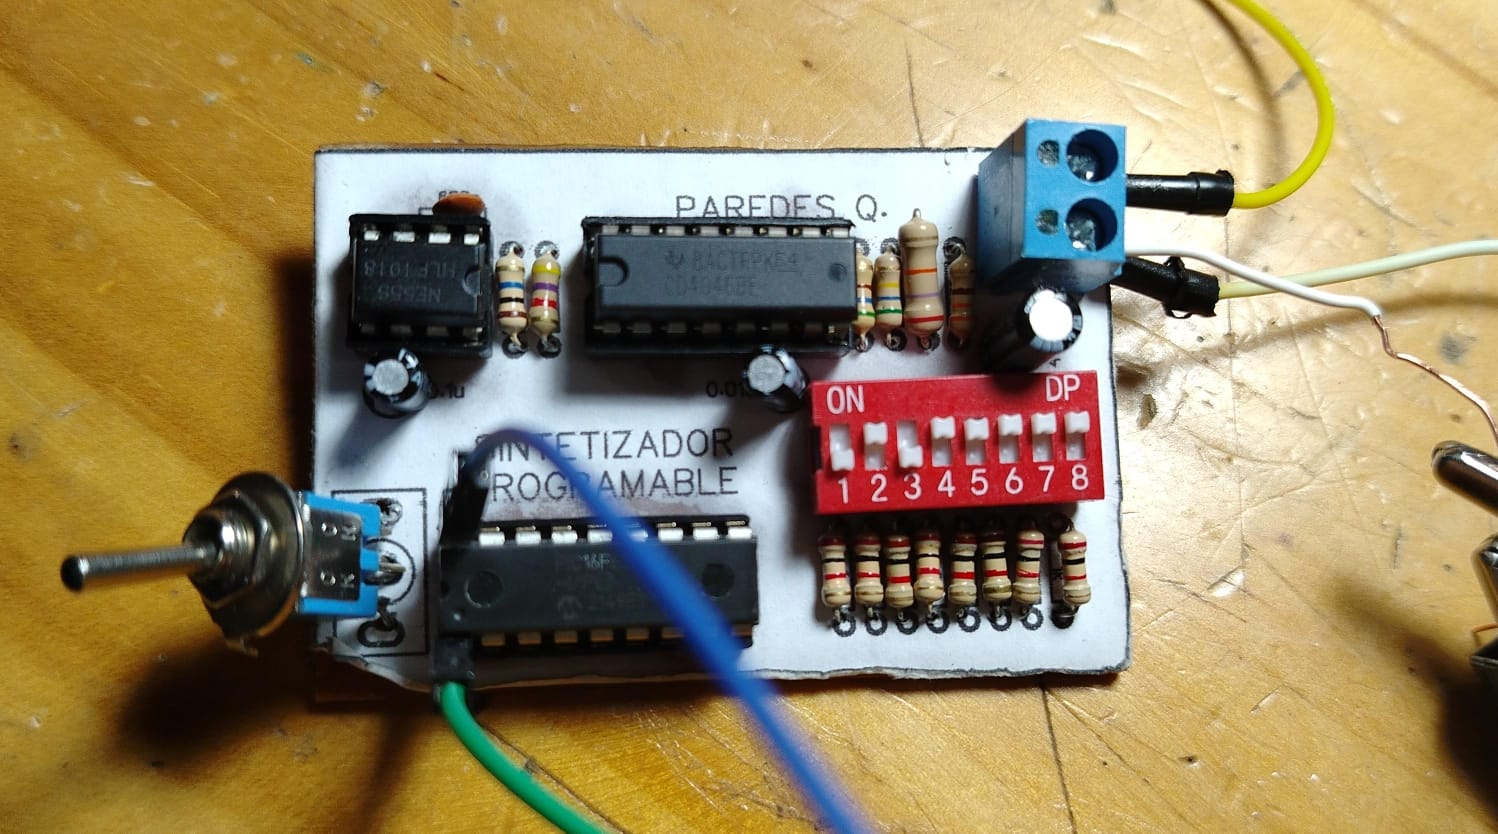
\includegraphics[width=.9\textwidth]{imgs/5.2. Cirucito con PIC.jpg}
        \caption{Sintetizador con un PLL y un PIC16F628A}
    \end{figure}
    \begin{figure}[H]
        \centering
        \includegraphics[width=.9\textwidth]{imgs/5.2. Salida PIC.jpg}
        \caption{Comparación entre la entada del demodulador de fase y el VCO (cambio cada 3 flancos)}
    \end{figure}
    \newpage
    \item Hacer un cambio de la amplitud de la señal de salida del oscilador, observar la salida y modificar hasta obtener la mejor señal de salida y anotar resultados de amplitud y frecuencia.
    \begin{figure}[H]
        \centering
        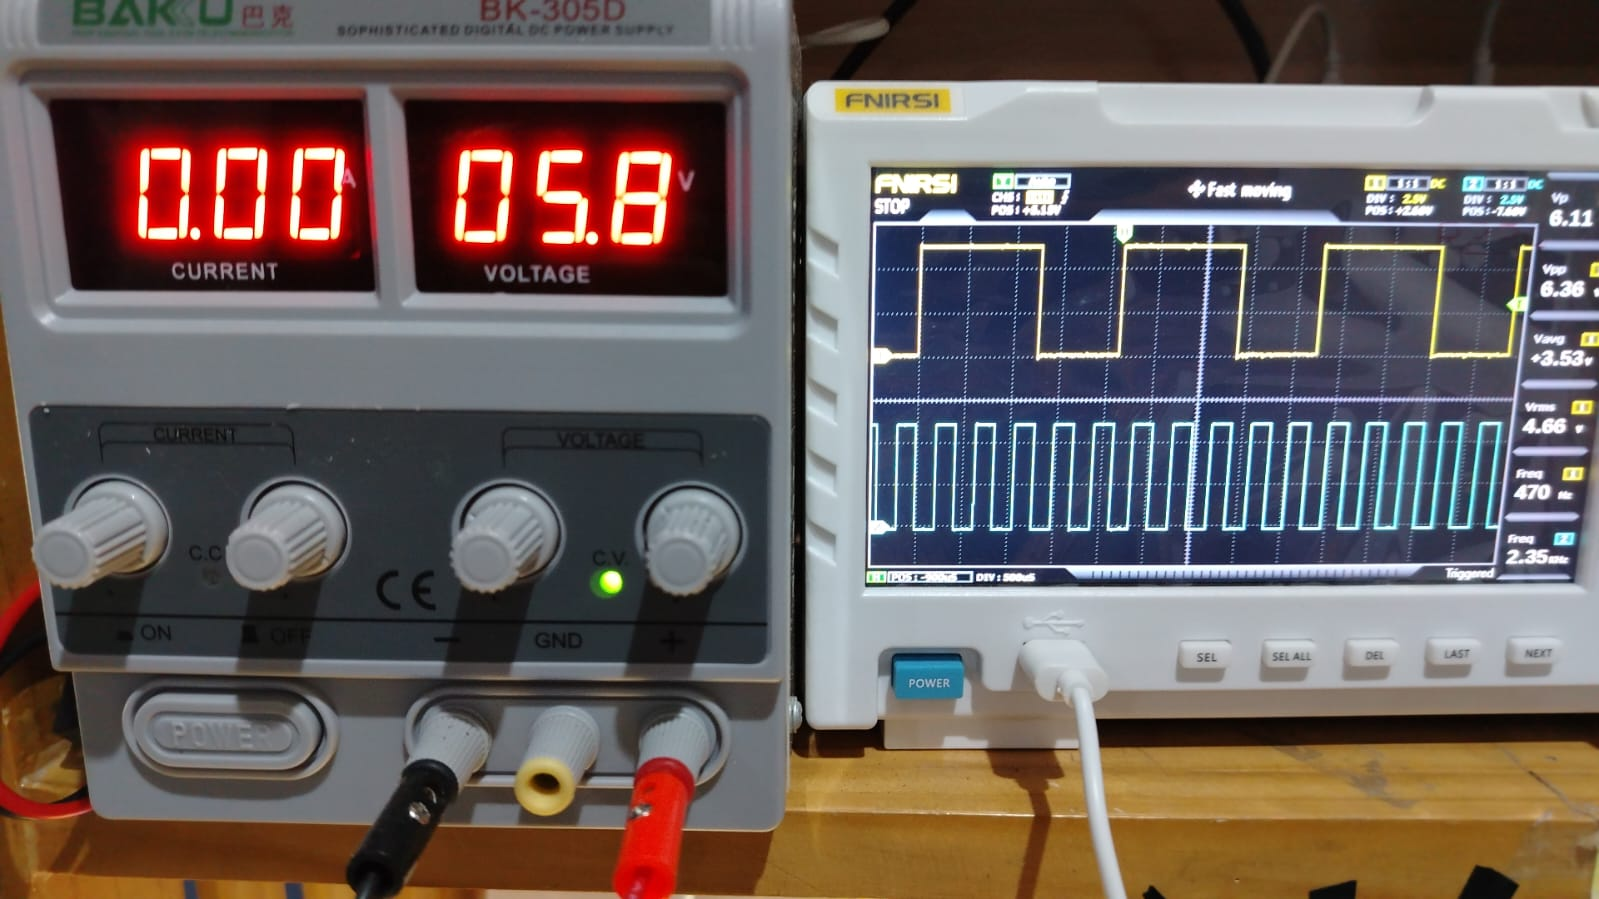
\includegraphics[width=.9\textwidth]{imgs/5.3. Nueva salida.jpg}
        \caption{Incremento de amplitud}
    \end{figure}
    Se incrementó la alimentación del sistema que dispone del 7493 (no se hizo esta variación en el sistema del PIC por cuidar el microcontrolador), lo condujo a un incremento de la amplitud de la salida del oscilador. Como se observa, todas las señales variaron en su amplitud pero no en frecuencia ni fase.
    \item Modificar el circuito contador para una división de menor valor.
    \begin{figure}[H]
        \centering
        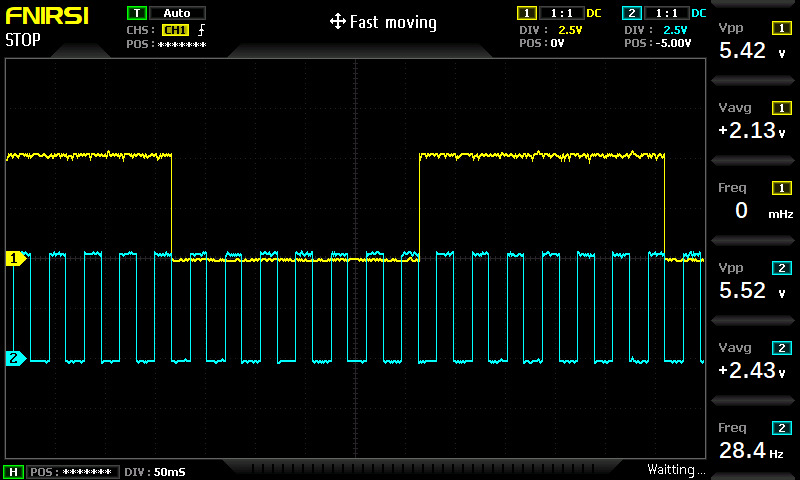
\includegraphics[width=.8\textwidth]{imgs/5.5. Menos frecuencia.jpg}
        \caption{División con PIC, cuenta 1 flanco para cambiar de estado}
    \end{figure}
    \item Modificar el circuito contador para una división de mayor valor
    \begin{figure}[H]
        \centering
        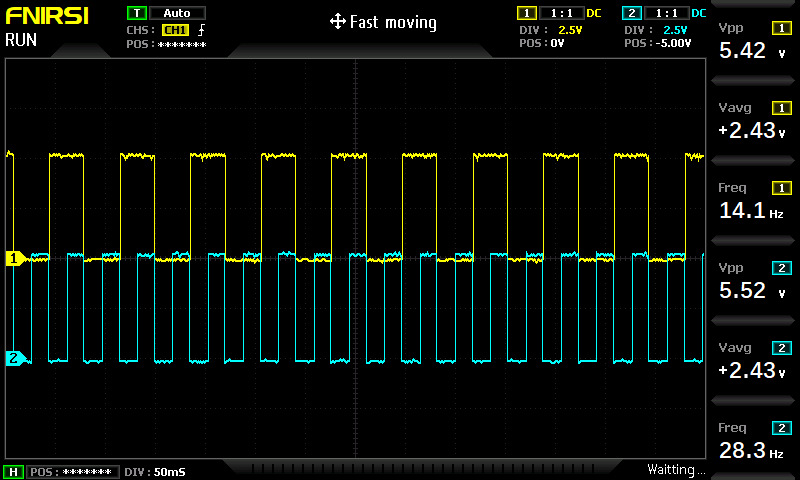
\includegraphics[width=.8\textwidth]{imgs/5.6. Más frecuencia.jpg}
        \caption{División con PIC, cuenta 7 flancos para cambiar de estado}
    \end{figure}
\end{enumerate}
